\documentclass[a4paper,norsk]{article}
\usepackage{preamble}
\usepackage{amsmath}
\begin{document}
\maketitle


As a strategy to approximate a function f with a function g ..  
\begin{align}
||f - g|| = \sqrt{\int_0^1 (f(t) - g(t) )^2 dt }	
\end{align} 
Further we define ${N_1(x), N_2(x), ..., N_n(x)}$ to be a basis for the set of polynomials of degree at most n-1. For a chosen set of basis, we want to 
find a "best fit" polynomial to f, such that $||\sum_{j=1}^n c_j N_j - f ||$ is minimized with respect to the coefficients $c_j$
From the least squares approximation, we end up with the system
\begin{align}
\mathbf{c^T N c} -2\mathbf{b^T c} + ||f||^2
\end{align}
Where \textbf{N} is the matrix with entries $\langle N_i, N_j \rangle$ and \textbf{b} is the vector with entries $\langle N_j, f \rangle$ 

\section*{Problem 1}
REWRITE AS HERMETIAN MATRIX!!
First we want to show that matrix \textbf{N} is positive definite.  A n × n real matrix M defined as positive definite if the scalar $ x^{T}M x$ is positive for every choice of a non-zero column vector x
x of dimention n. A natural extention of the definition would be to consider the system $\mathbf{c^TNc}$.
\begin{align}
c^TNc = c_i \langle N_i, N_j \rangle c_j = \int_0^1 \sum_{i=1}^n c_i N_i \sum_{j=1}^n c_j N_j dx = \int_0^1 p(x)^2 dx  \geq 0
\end{align}

\section*{Problem 2}
Computing the gradient of the expression $\mathbf{c^T N c} -2 \mathbf{b^t c} + ||f||^2 $ with respect to $c_i$ we get

\begin{align}
\frac{\partial}{\partial c_i} \mathbf{c^T N c} -2 \mathbf{b^t c} + ||f||^2 = 2\mathbf{Nc} - 2\mathbf{b^t} \\
\end{align}
From simple observations of the least squares method, one can see that the trend of $||f - g|| = \sqrt{\int_0^1 (f(t) - g(t) )^2 dt }$ will follow some sort of second order polynomial. Hence the minimal
extreme point for the smallest error will be found for $\frac{\partial}{\partial c_i} \mathbf{c^T N c} -2 \mathbf{b^t c} + ||f||^2 = 0$ hence $\mathbf{Nc} = \mathbf{b}$

\section*{Problem 3}
Defining $N_j(x) = x^{j-1} \hspace{2mm} 1 \leq j \leq n$, we are ought to show that the matrix \textbf{N} really is the Hilbert matrix with entries $\frac{1}{i + j - 1}$
\begin{align}
\mathbf{N} = \langle N_i, N_j \rangle = \int_0^1 x^{i - 1} x^{j - 1} dx = \int_0^1 x^{i + j- 2} dx = \Big[\frac{1}{i+j+1} x^{i+j+1} \Big]_0^1 = \frac{1}{i+j+1} 
\end{align}

\section*{Problem 4}
Showing that $P_n(x) = x^n + \sum_{k=0}^{n-1} c_k x^k$ is orthogonal to $1, x, ...., x^{n-1}$ on [-1, 1], we require that $\langle P_n,  N_j\rangle = 0$ \\
Since $\langle P_n,  N_j\rangle = 0$, then using the same arguments as in problem 3, we have to solve the linear system $\mathbf{Nc = b}$, where b in this will be a contribution from the $x^n$ term.
\begin{align}
\langle P_n,  N_j\rangle = \int_{-1}^1  \Big[x^n + \sum_{k=0}^{n-1} c_k x^k\Big]x^{j-1} dx = 0 \\
 \int_{-1}^1 \sum_{k=0}^{n-1} c_k x^k x^{j-1} dx = -\int_{-1}^1  x^n x^{-j} dx = -\langle x^n, x^{j-1}\rangle \\
 -\langle x^n, x^{j-1}\rangle = -\Big[\frac{x^{n+j} }{n+j} \Big]_{-1}^1  = 
 \begin{cases} 
      0 \hspace{2mm} \text{if n + j is even } \\
      -\frac{2}{n+j} \hspace{2mm} \text{if n + j is odd}
   \end{cases}
\end{align}

\section*{Problem 6}
\begin{figure}[h!]
	\centering
	\caption*{\textbf{First 10 Legendre polynomials}}
	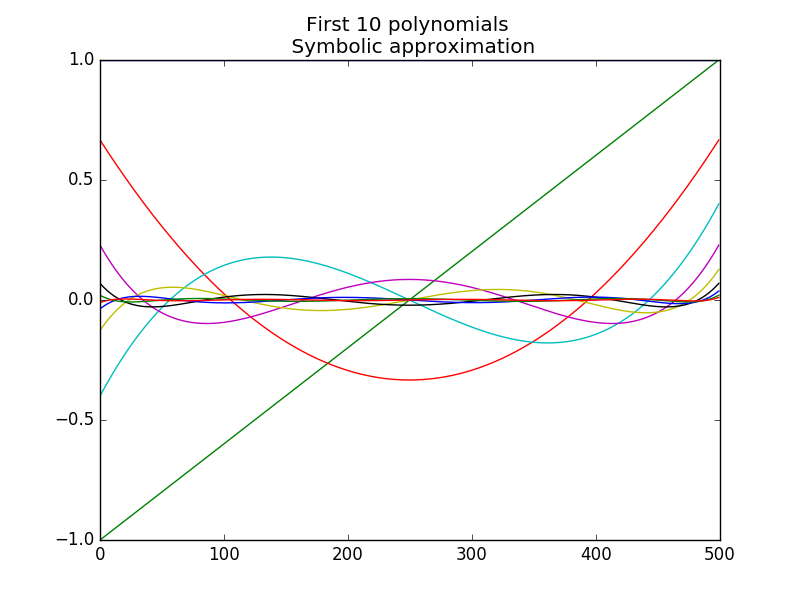
\includegraphics[scale=0.36]{sym10.png}
	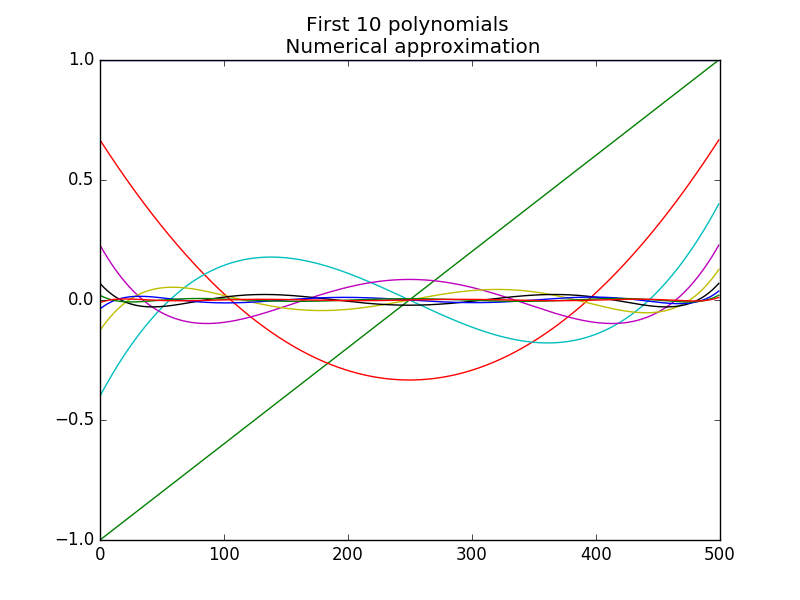
\includegraphics[scale=0.36]{num10.png}
\end{figure}

\section*{Problem 7}
\begin{figure}[h!]
	\centering
	\caption*{\textbf{First indication of trouble}}
	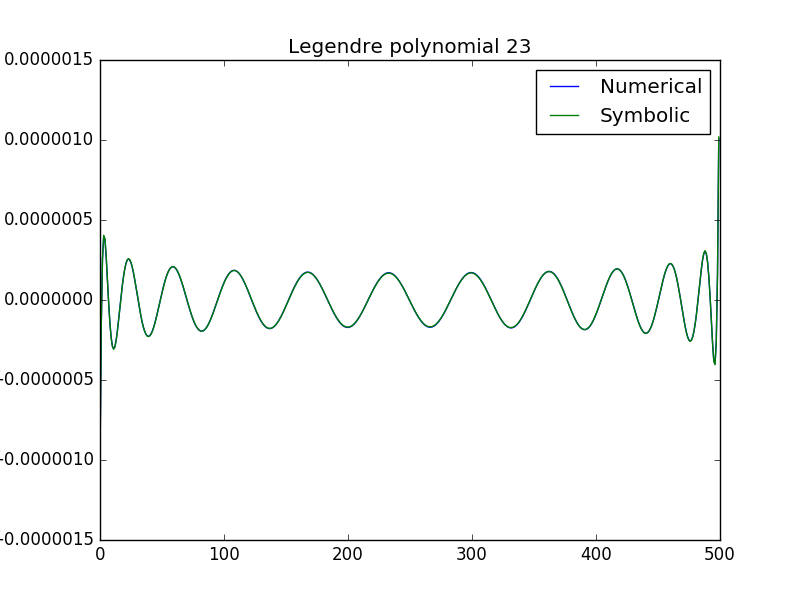
\includegraphics[scale=0.36]{n23.png}
	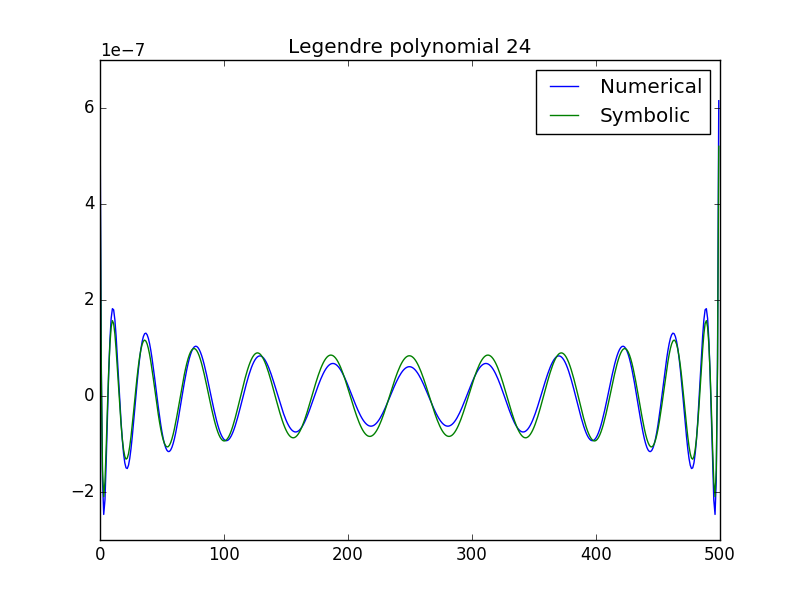
\includegraphics[scale=0.36]{n24.png}
\end{figure}

\end{document}

